\documentclass{report}
\usepackage{graphicx}
\usepackage[utf8]{inputenc}


\begin{document}

\begin{titlepage}


\center % Center everything on the page
 
\includegraphics[width=1.0\textwidth]{img/logos.png}

\vfill % Fill the rest of the page with whitespace

\textsc{\LARGE MOLUSCE}\\[1.5cm] 
\textsc{\Large Modules for Land Use Change Evaluation}\\[0.5cm] 
\textsc{\large Quick Help}\\[0.5cm]

\vfill % Fill the rest of the page with whitespace

 
\textsc{
License\\
Except where otherwise noted, content of this work is licensed under a Creative
Commons Attribution-ShareAlike 3.0 Unported~License.
}

\end{titlepage}


\tableofcontents


\chapter{Plug-in overview}
\section{Introduction}

Open source software platforms are progressively becoming widely used in the public and private
sectors. In Geographical Information System (GIS), open source software packages such as QGIS
are actively being developed. More importantly, customization and further development is possible
since developers create specific plug-ins with flexibility.

Asia Air Survey Co., Ltd. (AAS) started to move towards open source software since 2012
becoming the first QGIS gold sponsor worldwide. Furthermore, open source software started to be
used more extensively for internal use and in international project. Alongside with these recent
changes AAS also started to develop open source solutions aiming to further extend its market.


\section{What is MOLUSCE?}
AAS released MOLUSCE (Modules for Land Use Change Evaluation) at FOSS4G 2013.
MOLUSCE is a user-friendly plug-in for QGIS 3.0 and above. MOLUSE is designed to analyze,
model and simulate land use/cover changes. The plug-in incorporates well-known algorithms,
which can be used in land use/cover change analysis, urban analysis as well as forestry applications
and projects.

MOLUSCE is well suited to:
\begin{itemize}
  \item analyze land use and forest cover changes between different time periods;
  \item model land use/cover transition potential or areas at risk of deforestation; 
  \item and simulate future land use and forest cover changes
\end{itemize}


\section{Functions}
MOLUSCE user interface offers an easy-to-use interface with specific modules and functions.
Following is a brief description of basic modules in MOLUSCE.

\paragraph{Input module}
Land use/cover maps from different epochs, biophysical and socio-economic driving factor data
such as road network, rivers, topography, population etc., are loaded in the input module.

\paragraph{Area change analysis}
Computes land use/cover changes between two time periods (T1 and T2). Land use/cover change
transition matrices as well as land use change maps are produced.

\paragraph{Modeling methods}
Four methods, namely Artificial Neural Networks (ANN), Logistic Regression (LR), Multi-Criteria
Evaluation (MCE) and Weights of Evidence (WoE) are used for modeling land use/cover change
transition potential.

\paragraph{Simulation}
Displays transition potential maps, certainty function (experimental) and simulation results. A
simulated (projected) land use/cover map is produced based on a Monte Carlo Cellular-automata
modeling approach.

\paragraph{Validation}
This sub-module incorporates Kappa statistics (standard Kappa, Kappa histogram and Kappa
location), which will be used to validate the accuracy of the simulated land use/cover maps.

\chapter{How to use MOLUSCE}

\section{Inputs}
A screenshot of \verb+Inputs+ tab is shown in Figure~\ref{fig:inputs_tab}.

\begin{figure}[h!]
\centering
\includegraphics[width=0.95\textwidth]{img/inputs_tab.png}
\caption{Inputs tab}
\label{fig:inputs_tab}
\end{figure}

Data can be loaded using the inputs tab. To load your data follow the next steps (Figure~\ref{fig:inputs_tab}).

\begin{itemize}

  \item Step 1. Load all rasters that you need in the input tab. 
  \item Load the initial and final land use/cover maps as shown in steps 2 and 3. The base map determines
  the geometry of all the output files, pixel size, scaling and projection.
  \item Steps 4 and 5 show the corresponding years. (The user can type here If the corresponding years do
  not appear automatically).
  \item Steps 6 and 7 show how the add/remove buttons used to add or remove spatial variables.
  \item The selected spatial variables are shown in step 8.
  \item The check geometry button is a mandatory step to check if the geometry of the selected raster is
  matched (step 9).
\end{itemize}


Note: It is important when layers are added to QGIS that the No Data Value (NDV) is set. If this is
not done, MOLUSCE will process NDV areas as land use/cover classes, increasing processing time
and confusing the model calibration. MOLUSCE picks up the NDV of the input (base) layer and
propagates it to any output maps generated, along with the geometry of the base layer.\bigskip

Note: In the current version of MOLUSCE, it is essential that the initial and final LULC rasters contain the same set of unique class values. For example, if the initial raster includes the values 1, 2, 3, and 4, then the final raster must also contain exactly these values: 1, 2, 3, and 4. If a new class value appears or an existing one disappears during the transition, MOLUSCE will not be able to process the data. As a workaround, users can artificially adjust the sets of unique values to match. One approach is to use the free \textbf{Serval} plugin, which allows editing of raster pixel values. You can, for instance, add a single pixel with the missing class value in a corner of the raster. This small change will not significantly affect the transition analysis but will ensure that MOLUSCE can process your data.

\section{Evaluating correlation}

The \verb+evaluating correlation+ module contains three techniques for performing correlation analysis:
\begin{enumerate}
  \item Pearson's correlation.
  \item Cramer's coefficient.
  \item Joint information uncertainty.
\end{enumerate}

The user can choose between a two-way raster comparison by selecting \verb+first raster+ and \verb+second raster+
or \verb+check all rasters+ loaded into MOLUSCE.

\begin{figure}[h!]
\centering
\includegraphics[width=0.95\textwidth]{img/correlation_tab.png}
\caption{Evaluation correlation tab}
\label{fig:correlation_tab}
\end{figure}

The user can run correlation by pressing the \verb+check+ button located at the bottom of the window (see Figure~\ref{fig:correlation_tab}).

Note: The \verb+Cramer's coefficient+ and \verb+joint information uncertainty+ work only with categorical data.
The data should be converted to categorical data (eg. using GRASS).

\section{Area Changes}

A screenshot of \verb+Area Changes+ tab is shown in Figure~\ref{fig:changes_tab}.

\begin{figure}[h!]
\centering
\includegraphics[width=0.95\textwidth]{img/changes_tab.png}
\caption{Area Changes tab}
\label{fig:changes_tab}
\end{figure}

The \verb+update tables+ button produces \verb+class statistics+ and \verb+transition+ \verb+matrix+ tables.

The \verb+class statistics+ table shows the initial and final land use/cover change (LUC) areas.

The \verb+transition matrix+ shows the proportions of pixels changing from one land use/cover to another.

The \verb+create change map+ button will generate a map of change classes. This will be added
automatically to QGIS and saved as a GeoTiff.

Note: Data from tables can be copied and pasted directly into spreadsheet programs, simply by
selecting the desired rows/columns and by pressing the “Ctrl~+~C” keyboard combination.

\section{Transition potential modeling}
MOLUSCE uses Artificial Neural Network (ANN), Multi Criteria Evaluation (MCE), Weights of
Evidence (WoE) and Logistic Regression (LR) methods to model land use/cover transition
potential. The user can select a \verb+method+ from the drop down menu.


ANN, WoE and LR are machine learning models; they "look" at the training samples and try 
to find patterns that are "hidden" in the samples. However MCE is different: 
it is a model in which an expert (the user) describes the importance of factors
according to his/her knowledge of the domain area. After that, the expert's knowledge is transformed into
a computational model that estimates transition potentials.

The models are trained using samples, so the sampling process is important for the results, see~Section~\ref{subsec:sampling_modes} for the reference about sample modes.


\subsection{Artificial Neural Network (ANN)}
MOLUSCE uses full-connected Multi-Layer Perceprtron for modeling.
A screenshot of an example of \verb+ANN model settings+ is shown in Figure~\ref{fig:ann_model}.

\begin{figure}[h!]
\centering
\includegraphics[width=0.95\textwidth]{img/ann_model.png}
\caption{Transition potential modeling: ANN model}
\label{fig:ann_model}
\end{figure}

The \verb+define samples+ function specify number of samples and sampling mode. In addition, the
sampling points created can be saved and displayed.

\paragraph{Inputs} Five inputs are used to customize the ANN modeling:
\begin{itemize}
  \item The \verb+neighbourhood+ defines count of neighbour pixels around current pixel. Size=1 means 9
    pixels (3x3 region), size=2 means 25 pixels (5x5), etc.
  \item \verb+Learning rate+, \verb+momentum+ and \verb+max iterations number+ define parameters of learning. Big
    learning rate and momentum allow fast learning, but the learning process can be unstable
    (spikes on the graph). Small learning rate and momentum means stable but slow learning.
  \item \verb+Hidden layers+ input string takes a list of numbers: $N_1$, $N_2$,  \dots, $N_k$, where $N_1$ is number of
    neurons in 1st hidden layer, $N_2$ is number of neurons in 2nd hidden layer and so on, $N_k$ is the
    number of neurons of the last hidden layer (k-th layer). For example if the user types in the
    input string “2” then a network with 1 hidden layer and 2 neurons will be created. In order to
    create a network with 2 hidden layers the user should insert 2 numbers, such as “10 2”
    which will create a network with 10 neurons in the first hidden layer and 2 neurons in the
    second.
\end{itemize}


\paragraph{Outputs} The following outputs are proposed (for the current learning iteration):
\begin{itemize}
  \item The graph area. Contains errors of training and validation sets. It is the main information
about learning process. The graph can be edited and saved as image.
  \item The \verb+min validation overall error+ contains information about min reached error on validation
set of samples.
  \item The \verb+delta overall accuracy+ contains difference between min reached error and current error.
  \item The \verb+current validation Kappa+ shows the Kappa value.
\end{itemize}

The training process can be started by pressing on the \verb+train neural+ \verb+network+ button and stopped at any time
using the \verb+stop+ button.

Learning algorithm analyses the reached accuracy on training and validation sets of samples and
stores the best neural net in memory. The training process finishes when the \verb+maximum iteration number+ is
reached, and the best neural net will be used to produce transition potentials.

\subsubsection{How to train the model}
There are few parameters that can dramatically change quality of trained model. 
The main of them are:
\begin{itemize}
  \item ANN complexity (number of layers and neurons): complex models are more powerful, but training them properly is hard process, complex models require more samples to train etc. 
  \item learning rate and momentum: large values of learning rate allow to train quickly, but the training process may be unstable in this case; momentum helps stabilize the training.
  \item sample count: large sample count allows to train complex models, but the training becomes slow and requires more computer memory (which can be issue for large rasters).
\end{itemize}

So process of ANN training is a trial and error method: during the training the uses searches "good" parameters that lead to "good" model.
The training graph is the main tool that provide information about the training process and model quality.

Bellow we provide an example of ANN training, discuss some potential caveats and how to fix them.


\paragraph{Unstable learning} Figure~\ref{fig:ann_spikes} shows an example of unstable learning process: there are a lot of spikes on the graph.
Note that the learning rate is 0.1.

A stable training process is one of the necessary conditions for good ANN model: we can't expect 
to learn something useful if the  values of its parameters show dramatic changes with every iteration.

\begin{figure}[h!]
\centering
\includegraphics[width=0.95\textwidth]{img/ann_spikes.png}
\caption{ANN model: spikes on the graph (unstable training)}
\label{fig:ann_spikes}
\end{figure}

We can fix the issue if decrease the value of this parameter. Figure~\ref{fig:ann_spikes_fxd} shows 
that if we set learning rate to 0.001 the learning curves become smooth. The smooth form of 
lines for training and validation errors indicates a stable training process. This means that the
internal values of the parameters of ANN model do not change suddenly with every iteration. 


\begin{figure}[h!]
\centering
\includegraphics[width=0.95\textwidth]{img/ann_spikes_fxd.png}
\caption{ANN model: smooth learning curves}
\label{fig:ann_spikes_fxd}
\end{figure}


But we can see that the model isn't perfect (look at the Kappa and validation error).

\paragraph{Improving the quality} Validation error and Kappa show than the model is not perfect (see Figure~\ref{fig:ann_spikes_fxd}).

We can add a neuron for the hidden layer, it makes the net more complex. The learning curves are shown in Figure~\ref{fig:ann_2neurons}.
We can see that Kappa is not zero and validation error decreases. It means that the model is getting better. 

\begin{figure}[h!]
\centering
\includegraphics[width=0.95\textwidth]{img/ann_2neurons.png}
\caption{ANN model: better model with slight over-fitting}
\label{fig:ann_2neurons}
\end{figure}

What about the over-fitting? The model shows some over-fitting (there is some difference between validation and training errors) but it is not significant.

\begin{figure}[h!]
\centering
\includegraphics[width=0.95\textwidth]{img/ann_overfitting.png}
\caption{ANN model: over-fitting example}
\label{fig:ann_overfitting}
\end{figure}

To get an example of clearer over-fitting, set 12 neurons in the hidden layer. 
The result presented in Figure~\ref{fig:ann_overfitting}.

We can see that the training error is decreasing but the validation error is still nearly constant. It is clear signal about over-fitting.
To avoid it we have two choices:
\begin{itemize}
    \item decrease number of neurons;
    \item increase sample count.
\end{itemize}

Figure~\ref{fig:ann_final} shows training on 20,000 samples.

\begin{figure}[h!]
\centering
\includegraphics[width=0.95\textwidth]{img/ann_final.png}
\caption{ANN model: final example}
\label{fig:ann_final}
\end{figure}

We can see that the training and validation errors are close. Over-fitting is not present.

\subsection{Multi Criteria Evaluation (MCE)}

The MCE model \cite{eastman1999multi} takes into account the expert point of view regarding the importance of the predictors. 
The user makes pairwise comparisons of the factors and describes their importance for the transition potentials. 
The comparisons are made using Saaty's scale (see~Table~\ref{tab:saaty_scale}).

\begin{table}
\centering
\caption{Saaty's scale}
\begin{tabular}{ll}
 \bf{Rating} & \bf{Preference}   \\
 1 & Equal importance  \\
 3 & Moderate importance \\ 
 5 & Strong importance \\
 7 & Very strong importance \\
 9 & Extreme importance \\
 2, 4, 6, 8 & Intermediate values 
\end{tabular}
\label{tab:saaty_scale}
\end{table}

For example, coefficient "1" between factors $A$ and $B$ means that the factors have equal importance for the transition process. 
Coefficient "9" between factors $A$ and $B$ means that factor $A$ absolutely exceeds factor $B$ in importance.

\begin{figure}[h!]
\centering
\includegraphics[width=0.95\textwidth]{img/mce_model.png}
\caption{Transition potential modeling: MCE model}
\label{fig:mce_model}
\end{figure}

A screenshot of an example of \verb+MCE model settings+ is shown in Figure~\ref{fig:mce_model}.

The user can set the values inside the \verb+pairwise comparison matrix+. 

The user can also select which classes to use to train the model by changing the \verb+from class+ 
and \verb+to class+ values located at the bottom of the window.


The model can be started by pressing the \verb+train model+ button.

The weights of the spatial variable will then appear in the \verb+weights matrix+.


\subsection{Weights of Evidence (WoE)}
The WoE \cite{bonham1989weights} method proposes two ways of defining the range breaks. 
The user can define a \verb+number of intervals+ or specify the 
\verb+range breaks+ values.

When the \verb+calculate range breaks+ button is pressed the weights information for each transition are
produced.

Once the user is satisfied with the weights the \verb+train model+ button can then be pressed.

\begin{figure}[h!]
\centering
\includegraphics[width=0.95\textwidth]{img/woe_model.png}
\caption{Transition potential modeling: WOE model}
\label{fig:woe_model}
\end{figure}

An example of WoE model settings is shown in Figure~\ref{fig:woe_model}.

\subsection{Logistic Regression (LR)}

An example of LR model settings is shown in Figure~\ref{fig:lr_model}.

\begin{figure}[h!]
\centering
\includegraphics[width=0.95\textwidth]{img/lr_model.png}
\caption{Transition potential modeling: LR model}
\label{fig:lr_model}
\end{figure}

The LR method offers the possibility to \verb+define samples+ (number of samples and sampling mode) as
well as save and display the sampling points created.

\paragraph{Inputs} Two inputs are used to customize the LR modeling:
\begin{itemize}
  \item The \verb+maximum iteration+ defines the total number of iterations.
  \item The \verb+neighbourhood+ defines count of neighbour pixels around current pixel. Size=1 means 9
pixels (3x3 region), size=2 means 25 pixels (5x5), etc.
\end{itemize}

\paragraph{Outputs} 

The following outputs are proposed (for the current learning iteration):

\begin{itemize}
  \item The \verb+pseudo R-squared+ shows the goodness-of-fit.
  \item The \verb+coefficients+ tab.
  \item The \verb+standard deviations+ tab.
  \item The \verb+p-values+ tab.
\end{itemize}

The user can run the model by pressing on the \verb+fit model+ button.

Note: For additional information on the LR outputs please consult the “Technical information:
Methods and Algorithms” manual.

\section{Saving and loading models}

Since version 5 it is possible to save the trained model to file (.molusce) and load models from files. Corresponding buttons are available at \verb+transition potential+ modeling tab, right to model type selector.

\begin{figure}[h!]
	\centering
	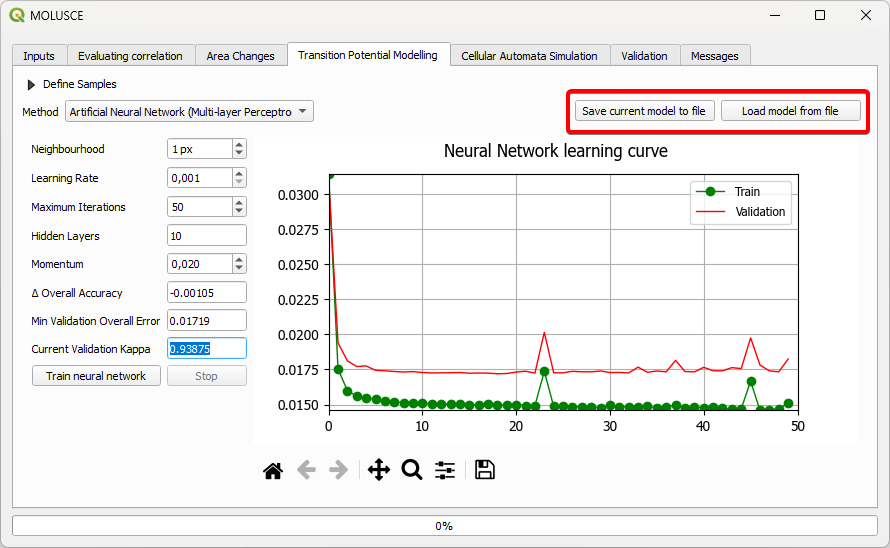
\includegraphics[width=0.95\textwidth]{img/saveload_buttons.png}
	\caption{Model save and load buttons}
	\label{fig:saveload_buttons}
\end{figure}

It is possible to save model of any type after fitting process is finished.

To load model, it should be ensured that:
\begin{itemize}
	\item Loaded model was trained on the data having same spatial domain (raster size, extent, coordinate reference system) as in current Inputs context.
	\item It was trained using the same number of spatial variables, having the same number of bands.
\end{itemize}

After loading the model log appears, containing information about loaded model. If it is incompatible with current Inputs setup, corresponding information is highlighted, as shown at Figure~\ref{fig:loaded_model_success} and Figure~\ref{fig:loaded_model_fail}.

After successful model import it is possible to proceed simulation.

\begin{figure}[h]
	\centering
	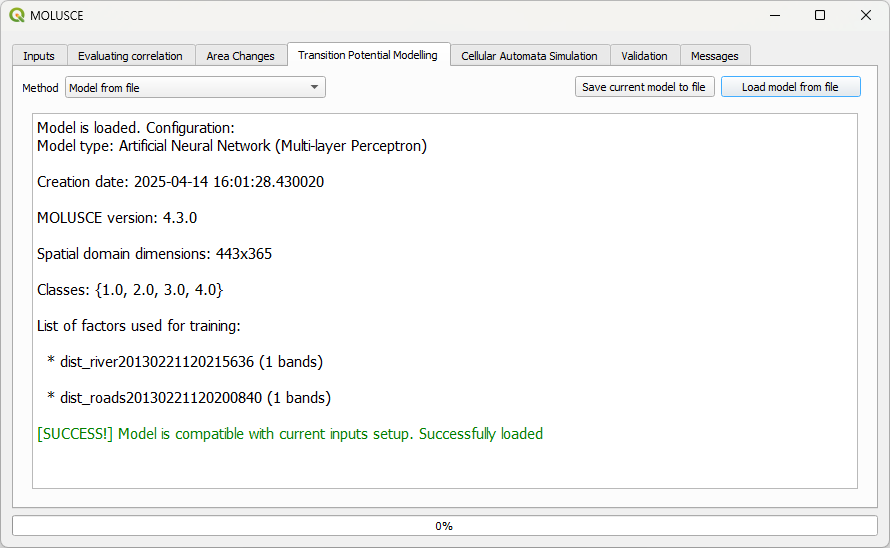
\includegraphics[width=0.95\textwidth]{img/loaded_model_success.png}
	\caption{Successfully loaded model info}
	\label{fig:loaded_model_success}
\end{figure}

\begin{figure}[ht!]
	\centering
	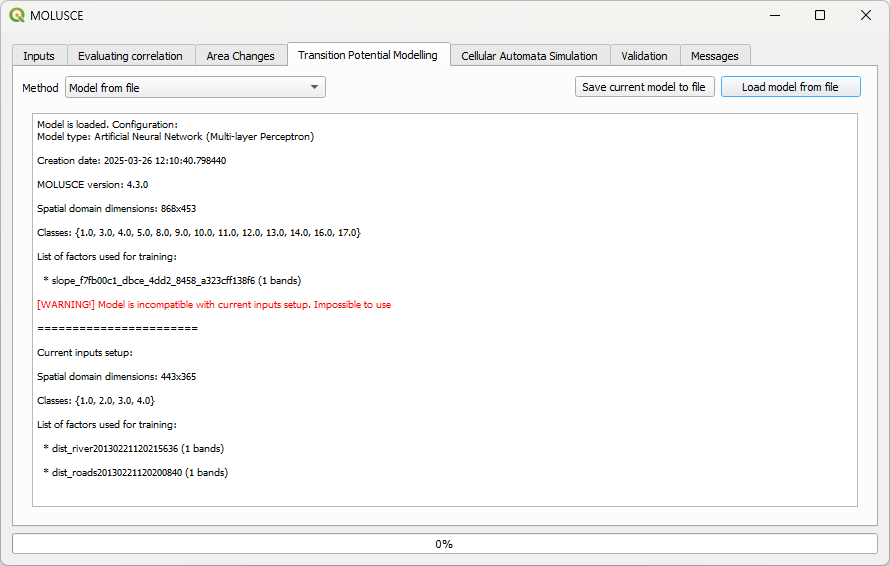
\includegraphics[width=0.95\textwidth]{img/loaded_model_fail.png}
	\caption{Failed model import info}
	\label{fig:loaded_model_fail}
\end{figure}

\section{Cellular Automata Simulation}

Once one method has been chosen and trained from the \verb+transition potential+ modeling tab, 
the user can then access to the \verb+cellular automata+ simulation tab.

\emph{Be aware that MOLUSCE will keep in memory the
latest method processed, if for example the user runs first the ANN and then the LR methods, the
cellular automata simulation tab will retain the results from the LR.}


\begin{figure}[h!]
\centering
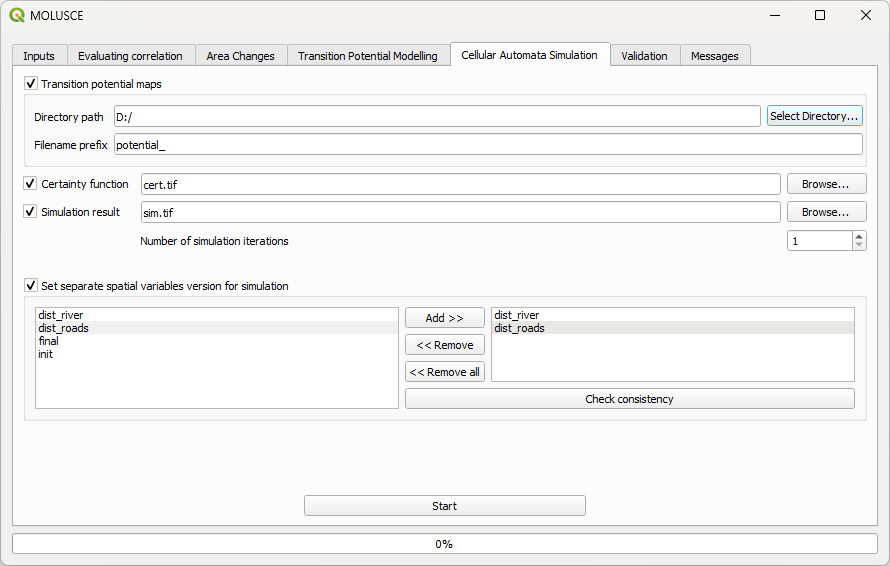
\includegraphics[width=0.95\textwidth]{img/simulation_tab.png}
\caption{Simulation tab}
\label{fig:simulation_tab}
\end{figure}

Three type of output maps are produced. A check box at the beginning of each output is provided to
allow the user to enable only what it is necessary. A \verb+browse...+ button located at the end of each
output allows to save each map.

\begin{itemize}
  \item The \verb+prefix of transition potential maps+ button allows to select prefix of the names of
    transition potential maps. Transition potential map shows the probability or potential to
    change from one land use/cover class to another. Transition potential values range from 0
    (low transition potential of change) 100 (high transition potential). Transition potential maps
    will be produced from the corresponding land use/cover changes (e.g., “forest to unstocked
    forest” transition potential, “forest to non-forest transition potential).
  \item The \verb+certainty function+.
  \item The \verb+simulation result+ produces a simulated land use/cover map.
\end{itemize}

An example of simulation tab is shown in Figure~\ref{fig:simulation_tab}.

Since version 5 it is also possible to set separate spatial variables version for simulation. This mechanism allows to address changing environment conditions influencing land cover dynamics, e.g. climate change, urbanization etc. To set up separate spatial variables version it is needed to activate corresponding checkbox and select new set of items.

\emph{It is crucial for new set of spatial variables to have the same number of records and their order as Input spatial variables. After selecting new items, Check consistency button should be pressed to run process of checking compatibility between Input variables and newly set variables.}

\section{Validation}

The \verb+validation+ tab allows the user to check, validate and compare the simulation results. 
\verb+Reference+ and \verb+simulated land use/cover maps+ must be loaded in order 
to start the validation process. The
former indicates a land use/cover map ($T_3$). $T_1$ refers to the initial land use/cover, while $T_2$ refers to
the final land use/cover used in the model). A \verb+browse+ button located at the end of each output
allows to load the desired map. A two way map comparison is performed from reference land
use/cover ($T_3$) and simulated land use/cover maps.

In order to perform a three way map comparison, the user can check the \verb+risk class validation map+
check-box. Although it is not shown explicitly, the three-way map comparison uses the initial land
use/cover map ($T_1$), the reference land use/cover map ($T_3$) and the simulated land use/cover map.

The \verb+multiple-resolution budget+ method~\cite[Chapter~17]{pontius2004maps_aggreament} is also used in MOLUSCE. The user can decide the 
\verb+number of validation iterations+ and can start the process by pressing the \verb+start validation button+.
The graph can be edited and saved as image.

The overall accuracy (\verb+% of correctness+, \verb+Kappa (overall)+, \verb+Kappa (histo)+ and \verb+Kappa (loc)+) can be
executed by clicking the \verb+calculate Kappa+ button.

\begin{figure}[h!]
\centering
\includegraphics[width=0.95\textwidth]{img/validation_tab.png}
\caption{Validation tab}
\label{fig:validation_tab}
\end{figure}

An example of validation tab is shown in Figure~\ref{fig:validation_tab}.
We discuss here some parts of the graph, see full details in~\cite[Chapter~17]{pontius2004maps_aggreament}.
The chapter propose 15 types of statistic, but MOLUSCE calculates and plots 5 of the most important of them:
\begin{itemize}
  \item No location information, no quantity information;
  \item No location information, medium quantity information;
  \item Medium location information, medium quantity information;
  \item Perfect location information, medium quantity information;
  \item Perfect location information, perfect quantity information.
\end{itemize}

These lines agreement metrics. They are measured for maps at different scales. 
The zero point on the abscissa axis corresponds to
the original scale of the maps, the point one corresponds the maps scaled down by half ($2^1$), the point
two corresponds the maps scaled down by quarter ($2^2$), etc.

Medium location information, medium quantity information is "the main" line.
It represents sequence of measures of agreement between the reference map and the simulated map.
Higher values of the line show higher agreement.

Other lines show  measures of agreement between the reference map and those that describe different hypothetical situations.
For example the line "No location information, no quantity information"  is the agreement due to chance.
Usually it lies below the "Medium-Medium" line, in this case the simulated map has better agreement with the reference 
then random generated map.

The upper line, "Perfect-Perfect," represents the highest possible agreement.
It corresponds to the case when we have complete information about the reference map in advance 
and can place all changes in their correct locations during the simulation.
Thus, this line shows the case when no errors are committed.
Usually the "Medium-Medium" line lies below this line.

Other lines represents other hypothetical situations when we know more or less information
about the reference map. This information consists of two parts: information about the quantity of pixels (quantity of changes in our case)
and information about the locations of changes.


\chapter{Technical details}
This chapter describes some algorithm and math details used for QGIS MOLUSCE plugin.
In this chapter we use the next terminology:
\begin{description}
\item[A model] is an algorithm that is used for predicting land use changes (transitions).
\item[A state] raster is a one-band raster where each pixel is assigned a land use category.
\item[The input state] raster is a one-band raster describing the past.
\item[The output state] raster is a one-band raster describing the present. It is the desired result of the prediction for the model (a user trains the model to predict (input raster, factors) -> output raster).
\item[A factor] raster is a raster of explanatory variables. The rasters can be one-band or multi-band.
\item[A transition class,] or simply transition,' is information about land use change.
  Every change (for example, forest --- non-forest) can be viewed as a transition of land use categories (encoded as pixels) from the input state raster to the output state raster.
\item[A change map] is an integer one-band raster that stores information about transitions.
  The category values of the change map are mapped one-to-one to transition classes.
\end{description}

The user declares the input and output state rasters, as well as the factor rasters, via the GUI.

\section{Data types}

The next assumptions are currently used by the plugin:
\begin{itemize}
    \item Initial and final state rasters are categorical one-band rasters; therefore a change map is categorical one-band raster too (see Section~\ref{sec:changemap_encoding}).
    \item For the ANN, MCE, and LR models, factor rasters are assumed to be ordinal or continuous (one-band or multi-band), but not categorical.
      These assumptions are very important because categorical data requires dummy encoding (see Section~\ref{subsec:dummy_coding}),
      while ordinal and continuous data need normalization (see Section~\ref{subsec:normalization}).
\end{itemize}
    
\section{Change map and area analysis}\label{sec:changemap_encoding}

\begin{table}[]
\centering
\caption{Change map encoding schema}
\begin{tabular}{rcccc}
           & \bf{Category 1} & \bf{Category 2} & \dots & \bf{Category N} \\
\bf{Category 1} & 0          & 1          & \dots  & N-1          \\
\bf{Category 2} &  N         & N+1        & \dots  & 2N-1       \\
 \dots     &  \dots     &   \dots    & \dots  &   \dots  \\
\bf{Category N} &  (N-1)*N   & (N-1)*N + 1 & \dots  &  N*N -1          
\end{tabular}
\label{tab:changemap_encoding}
\end{table}

The output of the Area Analysis stage is a change map; it is a raster where each pixel is assigned an integer value indicating its transition.
The module uses the following scheme for transition encoding (see Table~\ref{tab:changemap_encoding}).

For example, for 4 classes (N=4), there are 4*4=16 possible transitions (see Table~\ref{tab:changemap_encoding_example}).  
For example, if in the state rasters category "Forest" coded as "2", category "Urban" coded as "3", then transition "Forest" - "Urban" in the change map will be coded as "6". 

\begin{table}[]
\centering
\caption{Change map encoding example}
\begin{tabular}{rcccc}
           & Agriculture (1) & Forest (2) & Urban (3) & Water (4) \\
Agriculture (1) & 0          & 1          & 2  & 3          \\
Forest (2) &  4         & 5        & 6  & 7       \\
Urban (3) &  8     &   9    & 10  &   11  \\
Water (4) &  12   & 13 & 14  &  15          
\end{tabular}
\label{tab:changemap_encoding_example}
\end{table}
One row (in this case it is Water) consists of zeros.
It is important because otherwise the dummy variables became linear-dependent.
The condition of linear independence of data is crucial for Logistic regression and strongly recommended for Multilayer Percepton. 


\section{Sampling of points and data transformation}

Before the modeling stage some internal data transformations are made.
The transformations are not visible to the user, but understanding of them can help improve the quality of modeling results.

The transformations are made during data sampling stage.


\subsection{Dummy coding}\label{subsec:dummy_coding}
As the initial state raster and change map are categorical, each of them must be transformed to set of independent variables.

To do that the plugin uses dummy coding -- a categorical variable of N levels is divided into N-1 dummy variables. For example, if our land use map has 4 classes (Agriculture, Forest, Urban, Water), we have to use 3 dummy variables (see Table~\ref{tab:dummy_coding_example}). 

\begin{table}[]
\centering
\caption{Dummy coding example}
\begin{tabular}{rccc}
           & Dummy (1) & Dummy (2) & Dummy (3) \\
Agriculture & 0    & 0         & 1  \\
Forest&  0        & 1        & 0  \\
Urban &  1         &   0      & 0 \\ 
Water &  0         & 0        & 0            
\end{tabular}
\label{tab:dummy_coding_example}
\end{table}

One row (in this case it is Water) consists of zeros.
This is important because otherwise the dummy variables became linear-dependent.
The condition of linear independence of data is crucial for Logistic regression and strongly recommended for Multilayer Percepton. 



\subsection{Normalization}\label{subsec:normalization}
The next stage of initialization/sampling procedure is normalization of factor data. Usually normalization allows to achieve more efficient training and more accurate prediction result. The plugin uses linear normalization:
$$
X_{norm} = \frac{X-m_x}{\sigma_x}.
$$

Here $X$ is our variable, $X_{norm}$ is the normalized variable, $m_{x}$ is mean of X and $\sigma _{x}$ is standard deviation of $X$. 

Note that MCE method uses slightly different normalization (see~Section~\ref{subsec:MCE}).


\subsection{Sampling process}\label{subsec:sampling}

Sampling procedure processes single pixels and a neighborhood of pixels.
This means that a user can take into account a set of pixels around current pixel.
The implementation of the algorithm uses Moore neighborhood.

\begin{figure}[h!]
\centering
\includegraphics[width=0.95\textwidth]{img/neighbourhood_example.png}
\caption{Example of three neighbourhoods: 0-size (a pixel), 1-size and 2-size.}
\label{fig:neighbourhood_example}
\end{figure}

For example (see~Figure~\ref{fig:neighbourhood_example}), if the user sets up 1-size neighborhood then sampling procedure reads the current pixel and all pixels located in immediate vicinity (3x3 window size). If the user set up 2-size neighborhood then sampling procedure reads the current pixel and all pixels located in 5x5 window size and so on. Every neighborhood is stored as vector (9 elements, 25 elements and so on). Sampling is performed for every input raster (initial state raster and factors).

Thus a sample contains:
\begin{itemize}
    \item coordinates of the pixel (the coordinates doesn't used during training processes, they are used in some internal parts of the plugin),
    \item input data; that is used as input for models (for training and inference stages), the data consists of 2 parts:
      \begin{itemize}
      \item state pixel vector is the neighborhood that is read from 1-band raster, this raster contains initial states (categories). The raster is divided into set of dummy variables before sampling (see~Section~\ref{subsec:dummy_coding}).
        \item factor pixel vectors are the neighborhoods extracted from factor rasters (they can be multiband); every raster band is normalized before sampling (see~Section~\ref{subsec:normalization}).
      \end{itemize}
    \item output data is read from 1-band raster, this raster contains final states or the change map.
\end{itemize}

\subsubsection{Sampling modes}\label{subsec:sampling_modes}
The plugin has three sampling modes:
\begin{description}
    \item[All.] This mode extracts information for all pixels of the input and output rasters Among other methods this mode of sampling needs the biggest amount of RAM and CPU time
    \item[Random.] This mode extracts information for randomly selected samples: if raster has $N$ pixels, then the every pixel has equal ($\frac1N$) probability of being selected during sampling
    \item[Stratified.] This mode randomly undersamples major categories (large areas) and/or oversamples minor categories (small areas) If $C$ is desired count of samples and $K$ is number of output categories, then the sampling procedure select $K$ random groups of pixels of equal size $\frac{C}{K}$ Every group will contain pixels of one certain category
\end{description}

\section{Some words about modeling}\label{sec:modeling}

A user has a number of factors, init state raster and final state raster.
The goal of modeling stage is to create a model that can predict land use changes between those states. Before discussing prediction methods we need to explain common preparation stage.

\subsection{ANN: Multilayer perceptron}\label{subsec:ANN}

The plugin uses classic realization of Multilayer perceptron. The input data is a collection of pixels of initial state raster and factor rasters. The target output data is the change map.

So, the perceptron model performs the next actions:
\begin{enumerate}
    \item Initial preprocessing of the data (dummy coding and normalization).
    \item Sampling.
    \item Training.
\end{enumerate}

The initial stages are described (in general) in the previous sections (see~Sections~\ref{subsec:dummy_coding} and~\ref{subsec:normalization}), this subsection discussed the structure of the neural net, the training procedure and particular features of initialization. 

MOLUSCE uses multilayer percepron with \verb+numpy.tanh+ sigmoid function. Therefore target variables (the change map categories) should be scaled to $(-1, 1)$ interval during dummy coding instead of classic $(0, 1)$. This process is performed automatically during the preparation.

The user can set arbitrary number of hidden layers (one or more) and arbitrary number (one or more) of neurons in the layers.
Finally the created net has:
\begin{itemize}
  \item $(C-1)(2N+1)^{2}+B(2N+1)^{2}$ input neurons;
  \item about $M$ output neurons (it depends on sampling mode, see below);
\end{itemize}
here $C$ is the count of land use categories, $N$ is the neighborhood size specified by the user, $B$ is the summary band count of factor rasters (for example if two factors are one-band and three-band, then $B=4$). $M$ usually is a count of unique categories in the change map ($C^{2}$). But the count of output neurons can be less then $M$, it depends on the sampling mode. If mode "Random" is used, some small classes could be omitted during sampling procedure. 

The module uses classic backpropagation algorithm with momentum for the learning procedure. Weights correction are performed as:
$$
w(n+1)=r*dw(n)+m*dw(n-1),
$$
where $w$ is a vector of neuron weights, $dw$ is a vector of weights changes, $n$ is an iteration number, $r$ is learning rate, $m$ is the momentum value. 

Training set is divided in two parts: learning set (80\% of samples by default) and validation set (20\% of samples). 

The module uses on-line learning with stochastic: a random sample is selected from the learning set, the weights of the net are updated during forward/backward propagation.

A error of fitting (for a sample) is the average square error of partial outputs of the net:

$$
E = \frac{t_i - o_i}/d
$$

where $E$ is a sample error, $t_{i}$ is the target value of a output neuron for given sample, $o_{i}$ is the real output value of the neuron, $d$ is the count of output neurons. 

\subsection{Logistic regression}\label{subsec:lr}
Logistic regression model behavior is very similar to the ANN. The input data is a collection of pixels of initial state raster and factor rasters. The target output data is the change map.

So, the logistic regression model also performs the next actions: 
\begin{enumerate}
    \item Initial preprocessing of the data (dummy coding and normalization).
    \item Sampling.
    \item Training.
\end{enumerate}

The created model has M ($((C-1)(2N+1)^{2}+B(2N+1)^{2}+1)$ coefficients, but only $(M-1)((C-1)(2N+1)^{2}+B(2N+1)^{2})$ are independent. As before (see~Section~\ref{subsec:ANN}), $C$ is the count of land use categories, $N$ is neighborhood size specified by the user, $B$ is summary band count of factor rasters (for example if two factors are user one-band and three-band, then $B=4$). $M$ usually is count of unique categories in the change map $C^{2}$). $M$ depends on the sampling mode also (see~Section~\ref{subsec:ANN}). 

\subsubsection{Examples}
\paragraph{Example 1.}
For example we discuss coefficients of one transition class (transition from land use category 2 to land use category 3, for example). If we have four land use categories 1,2,3,4 and we select one one-band factor and we use 0-neighborhood, we have 5 coefficients per transition class:
\begin{itemize}
    \item $b_{0}$ is the intercept;
    \item $b_{1},b_{2},b_{3}$ are the coefficients of dummy variables of current landuse state (categories of the raster are coded as: 1 = (0, 0, 1); 2 = (0, 1, 0); 3 = (1, 0, 0); 4 = (0, 0, 0), see~Section~\ref{subsec:dummy_coding});
      $b_{4}$ is the coefficient of factor pixel (0-neighborhood).
\end{itemize}

\paragraph{Example 2.}
If we select two one-band factors, we have 6 coefficients per transition class:
\begin{itemize}
  \item $b_{0}$ is the intercept;
  \item $b_{1},b_{2},b_{3}$ are the coefficients of dummy variables of current landuse state;
  \item $b_{4}$ is the coefficient of the first factor (0-neighborhood).
  \item $b_{5}$ is the coefficient of the second factor (0-neighborhood).
\end{itemize}

\paragraph{Example 3.}
if we use 1-neighborhood and two one-band factors, we have 37 coefficients per transition class:
\begin{itemize}
  \item $b_{0}$ is the intercept;
  \item coefficients from $b_{1}$ thru $b_{27}$ are the coefficients of dummy variables of current landuse state: ( $b_{1}$, \dots, $b_{3}$ are dummy variables for the upper-left corner of 3x3 neighborhood window);
  \item coefficients from $b_{28}$ thru $b_{36}$ are the coefficients of the first raster pixels (1-neighborhood uses 9 pixels or 3x3 window);
  \item coefficients from $b_{37}$ thru $b_{45}$ are the coefficients of the second raster pixels.
\end{itemize}

\subsection{Weight of evidence}\label{subsec:WoE}

Initially Weight of Evidence method was developed to process binary variables, but the method was later modified in order to enable it to handle multiple categories of variables.
If the user uses rasters with continuous values, he/she has to transform them into categorical variables.

MOLUSCE implementation uses the next one modification. To handle continuous factors user must split raster values into several categories (range binning). The GUI has a form that allows to perform transformation into categorical variables. A compromise is needed here: if the user set up too many binning values, then a small amount of pixels might fall into a category and accuracy of statistical calculations will be poor; on contrary if the user set up few bins, which will lead to few of weights are formed, that leads to poor accuracy again.

In the binning form GUI doesn't display all of the used rasters: if a raster is already categorical, it doesn't need transformation and it doesn't appear in the form. Currently a simple procedure is used to decide if rasters as categorical: if a raster has more then \verb+MAX_CAT+ (=100) unique values, then the raster is supposed to be continuous, otherwise the raster is treated as categorical.

The WoE fitting procedure starts after the transformation continuous --- categorical.The change map is divided into series of binary maps (one map per a transition class), then the set of weights are estimated for every binary map. 

\subsection{Multi criteria evaluation}\label{subsec:MCE}

The goal of the method is to predict a transition class encoded in the change map. Factor rasters are input data, places where a transition occurs are target values. MCE takes pairwise comparison matrix of factors and calculates weights of every factor. This means, that a user must specify the comparison matrix for every transition class. But count of transition classes increases as $O(n^{2})$, where $n$ is count of landuse categories (for example if $n=4$, we have 16 transition classes). To specify all comparison matrices for all transitions is too long and boring, that's why the MCE model predicts one transition class only.

The method needs normalization of factor rasters: this implementation uses a linear combination of factors, therefore they should be transformed to $[0,1]$. The module uses the next transformation (it differs from ANN and LR normalization, see~Section~\ref{subsec:normalization}):
$$
X_{norm} = \frac{X-X_{min}}{X_{max} - X_{min}}
$$
where $X_{norm}$ is normalized raster value, $X$ is initial raster value, $X_{min}$ is the min value of the raster, $X_{max}$ is the max value of the raster. 

\section{Simulation}\label{sec:simulation}

Simulation module performs land use change evaluation procedure. It takes as input the next data:
\begin{itemize}
    \item Initial state raster;
    \item Factor rasters;
    \item Model.
\end{itemize}

Initial state raster contains information about current land use categories, factor rasters contain information about explanatory variables. Model is a predictor that calculates transition potentials in the condition of the factors and current land use.

So module doesn't uses implicit transition rules, it uses transition potentials generated by the models. The neighborhood effect is achieved if a model uses neighborhood during training, for example logistic regression has a coefficient for every neighbor and the coefficient affects the transition potential. If model doesn't uses neighborhood, Simulator takes into account only general patterns. 

The module works as follow scheme:
\begin{enumerate}
    \item Simulator takes transition probabilities from the transition matrix and calculates count of pixels that has to be changed (for every transition class);
    \item Simulator calls a model, pass to it initial state raster and factor rasters;
    \item The model scans pixels of the rasters (and its neighbors if the model uses neighborhood) and calculates transition potentials of every transition class;
    \item Simulator constructs a 'certancy' raster: the pixel of the raster are the difference between two most large potentials of correspondent pixels of transition potential rasters. As result the raster contains the model confidence: the bigger is difference, the bigger is confidence;
    \item Simulator constructs a raster of the most probable transitions: the pixels of the raster are the transition class with the biggest potential of transition. This raster is an auxiliary raster; it is used during the next stage;
    \item For every transition class Simulator searches in the raster of the most probable transitions a needed count of pixels with the greatest confidence and changes the category of the pixels. If confidence of two or more pixels are close, then random choice of the pixel is used.
\end{enumerate}

The described scheme is used if the user specified only one iteration of simulation. If several iterations have to be preformed, in general the scheme is the same, but initial state rasters are changed on the next iterations: the first simulated map is the initial state map for thy second iteration, the result of the second iteration is the initial states of the third iteration and so on. 


\section{Validation}\label{sec:validation}

Validation module allows to check accuracy of the simulation. MOLUSCE has three types of validation:
\begin{itemize}
    \item Kappa statistics;
    \item Error budget validation;
    \item Error map validation.
\end{itemize}

\subsection{Kappa}
The module calculates three types of kappa statistic.
Let
\begin{itemize}
  \item $c$ is count of raster categories,
  \item $p_{ij}$ is the $i,j$-th cell of contingency table,
  \item $p_{iT}$ is the sum of all cells in $i$-th row, $p_{Tj}$ is the sum of all cells in $j$-th column,
  \item $P(A)=\sum _{i=1}^{c}p_{ii}$,
  \item $P(E)=\sum _{i=1}^{c}p_{iT}p_{Ti}$,
  \item $P_{max}=\sum _{i=1}^{c}min(p_{iT},p_{Ti})$ 
\end{itemize}

In this case the kappa statistics can be defined by the next rules.

\paragraph{Kappa:}
$$
K={\frac {P(A)-P(E)}{1-P(E)}}
$$

\paragraph{Kappa location:}
$$
K_{loc}={\frac {P(A)-P(E)}{P_{max}-P(E)}}
$$


\paragraph{Kappa histogram:}
$$
K_{h}={\frac {P_{max}-P(E)}{1-P(E)}}
$$

\subsection{Error budget}
MOLUSCE uses Error Budget technique~\cite[Chapter~17]{pontius2004maps_aggreament}.
Currently the pdf can be found here: \verb+http://www.econgeography.org/~rpontius/pontius_suedmeyer_2004_rsgisaa.pdf+

\subsubsection{Error map}

MOLUSCE produces map of errors. This map contains information about false predictions in simulated raster. The error map can be constructed by compassion of simulated map and reference map. The errors of simulation are stored in the error map.

Error map creating procedure has two modifications: two map comparison case and three map comparison case. 

\paragraph{Two maps comparison case.}
This modification compares simulated map and reference map.

Traditional approach to two class (C1 and C2) problem uses three types of prediction statuses (see~Table~\ref{tab:2classET}): "hits, misses, false alarm".

\begin{table}
\centering
\caption{Two-class error table.}
\begin{tabular}{lcc}
   & \bf{Reference map C1} & \bf{Reference map C2}   \\
 \bf{Simulated map C1} & Hit & Misses \\
 \bf{Simulated map C2} & False alarms & Hit 
\end{tabular}
\label{tab:2classET}
\end{table}

But in case of N class problem the classification "hits, misses, false alarm" is not so good because the terms "Misses" and "False Alarms" became ambiguous: there are different types misses/false alarms between different classes.

MOLUSCE uses common N-class approach, when error map contains every transition type error marked by a particular color, "Hits" are transparent. The errors are coded as transitions in change maps (see~Section~\ref{sec:changemap_encoding}).

If a transition for a certain location was simulated correctly then the pixel is transparent (white color on the picture). If the transition was simulated incorrect, then the pixel is colored.

\paragraph{Three maps comparison case.}
This modification uses three rasters for checking: simulated map, reference map and initial map.

The same idea of comparison is used for checking persistent classes and simulation errors. Persistent classes are pixels that are constant in initial raster, reference raster and simulated raster. Such pixels are marked by a certain color, "Hits" are transparent and transition errors are marked as in the two-map comparison problem. 

\bibliographystyle{plain}
\bibliography{references}

\end{document}


% LocalWords:  MOLUSCE FOSS4G QGIS MOLUSE
